% Auto-generated figure blocks for outputs/thesis/figures/*.png .
% Requires \usepackage{graphicx}; upload the PNGs under figures/ in Overleaf.

\begin{figure}[ht]
\centering

\includegraphics[width=0.9\linewidth]{figures/base_models_indomain.png}
\caption{Base models $\times$ losses, in-domain}
\label{fig:base_models_indomain}
\end{figure}

\begin{figure}[ht]
\centering
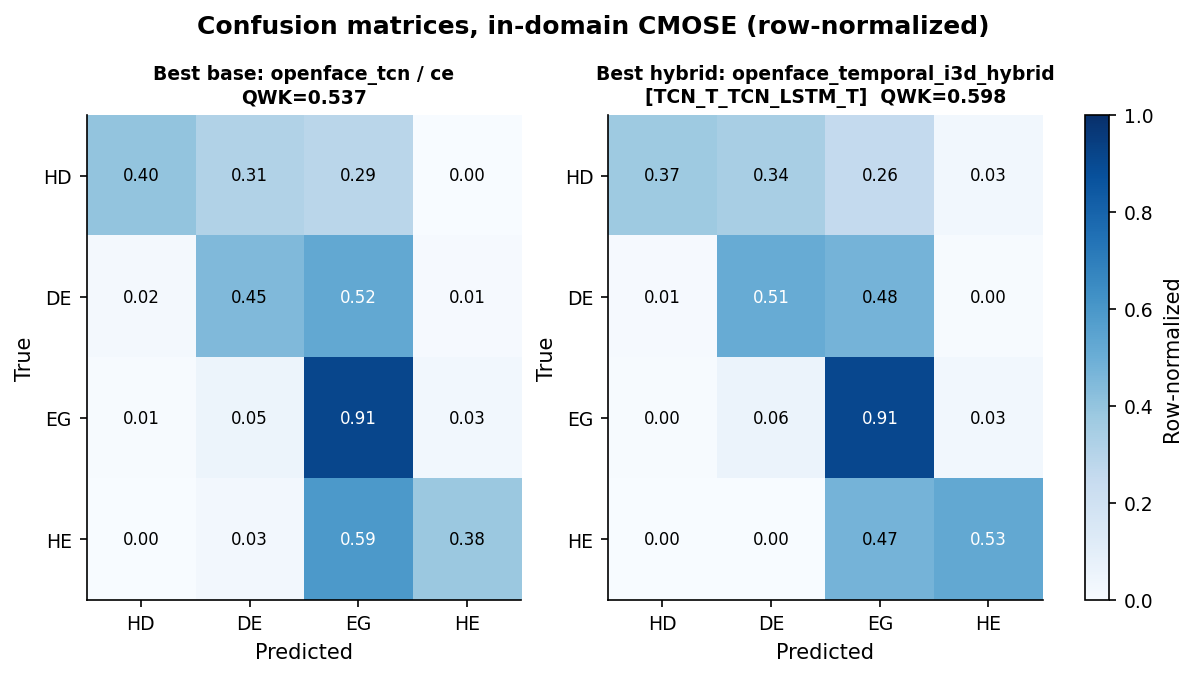
\includegraphics[width=0.9\linewidth]{figures/confusion_best_models.png}
\caption{Confusion matrices of best base vs best hybrid (in-domain)}
\label{fig:confusion_best_models}
\end{figure}

\begin{figure}[ht]
\centering

\includegraphics[width=0.9\linewidth]{figures/crossdomain_base.png}
\caption{Cross-domain generalization, best base model per cell}
\label{fig:crossdomain_base}
\end{figure}

\begin{figure}[ht]
\centering

\includegraphics[width=0.9\linewidth]{figures/crossdomain_hybrid.png}
\caption{Cross-domain generalization, best hybrid per cell}
\label{fig:crossdomain_hybrid}
\end{figure}

\begin{figure}[ht]
\centering
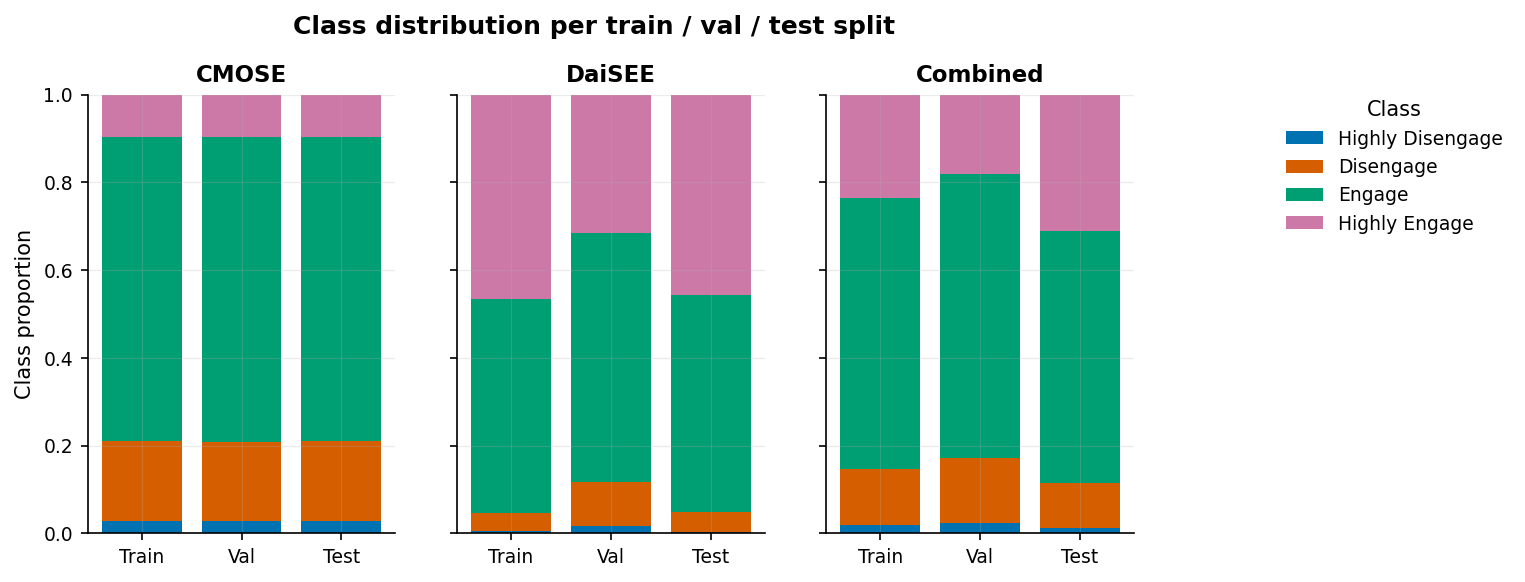
\includegraphics[width=0.9\linewidth]{figures/dataset_class_distribution_by_split.png}
\caption{Dataset class distribution by split}
\label{fig:dataset_class_distribution_by_split}
\end{figure}

\begin{figure}[ht]
\centering
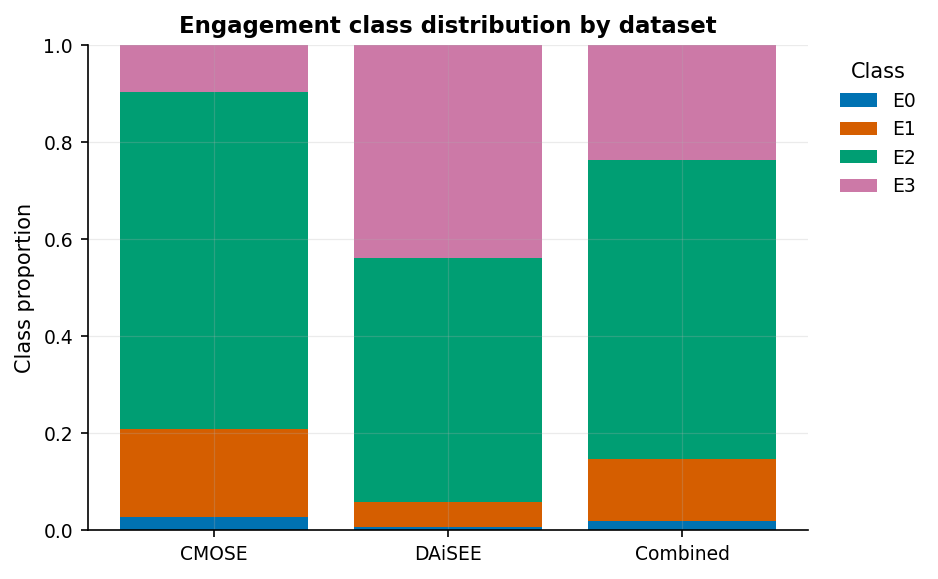
\includegraphics[width=0.9\linewidth]{figures/dataset_class_distribution_overall.png}
\caption{Engagement class distribution by dataset}
\label{fig:dataset_class_distribution_overall}
\end{figure}

\begin{figure}[ht]
\centering
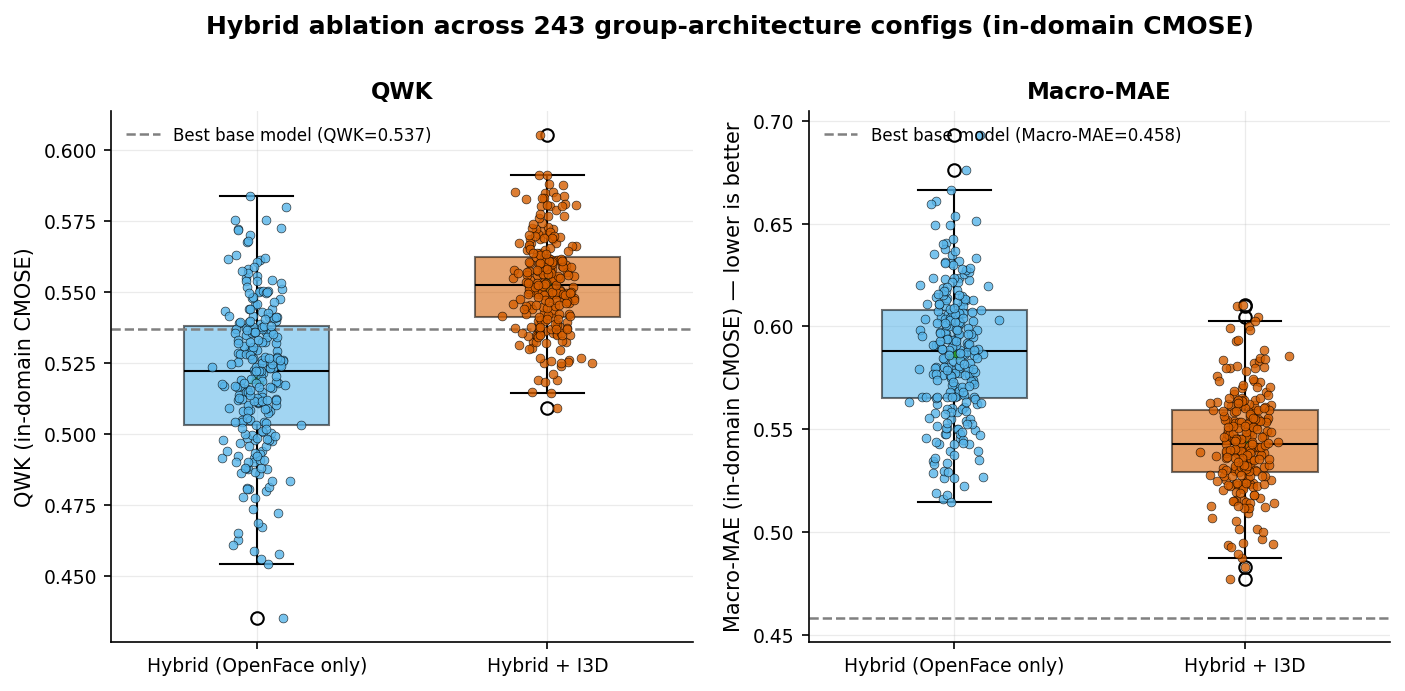
\includegraphics[width=0.9\linewidth]{figures/hybrid_ablation_distribution.png}
\caption{Hybrid ablation: QWK across 32 configs}
\label{fig:hybrid_ablation_distribution}
\end{figure}

\begin{figure}[ht]
\centering
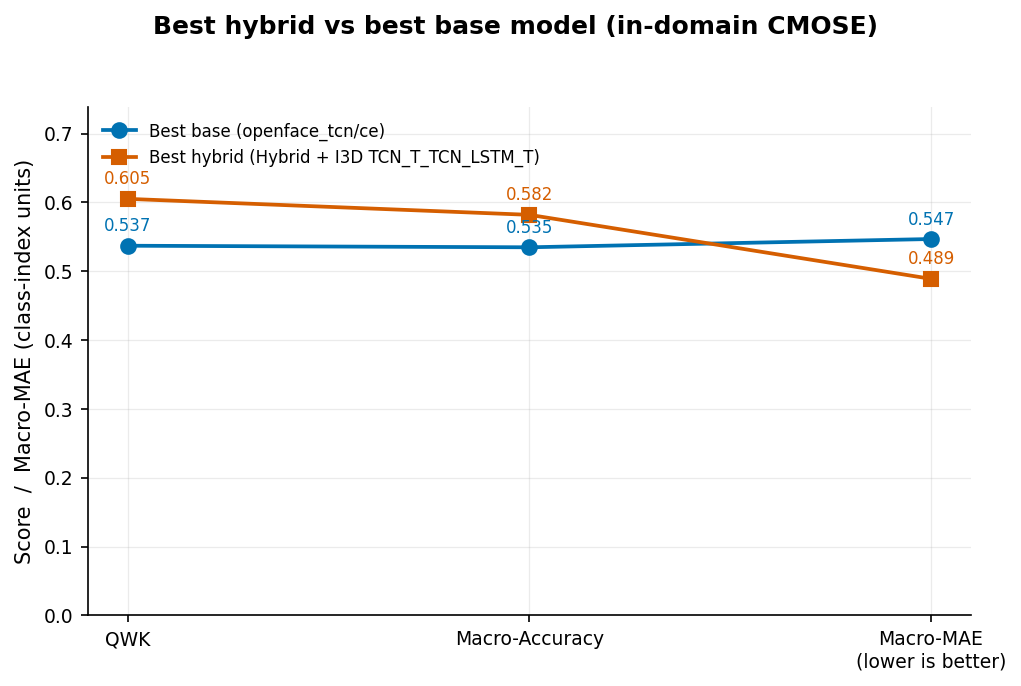
\includegraphics[width=0.9\linewidth]{figures/hybrid_best_comparison.png}
\caption{Best hybrid vs best base model}
\label{fig:hybrid_best_comparison}
\end{figure}

\begin{figure}[ht]
\centering

\includegraphics[width=0.9\linewidth]{figures/hybrid_group_marginal.png}
\caption{Per-group marginal effect of encoder choice}
\label{fig:hybrid_group_marginal}
\end{figure}

\begin{figure}[ht]
\centering
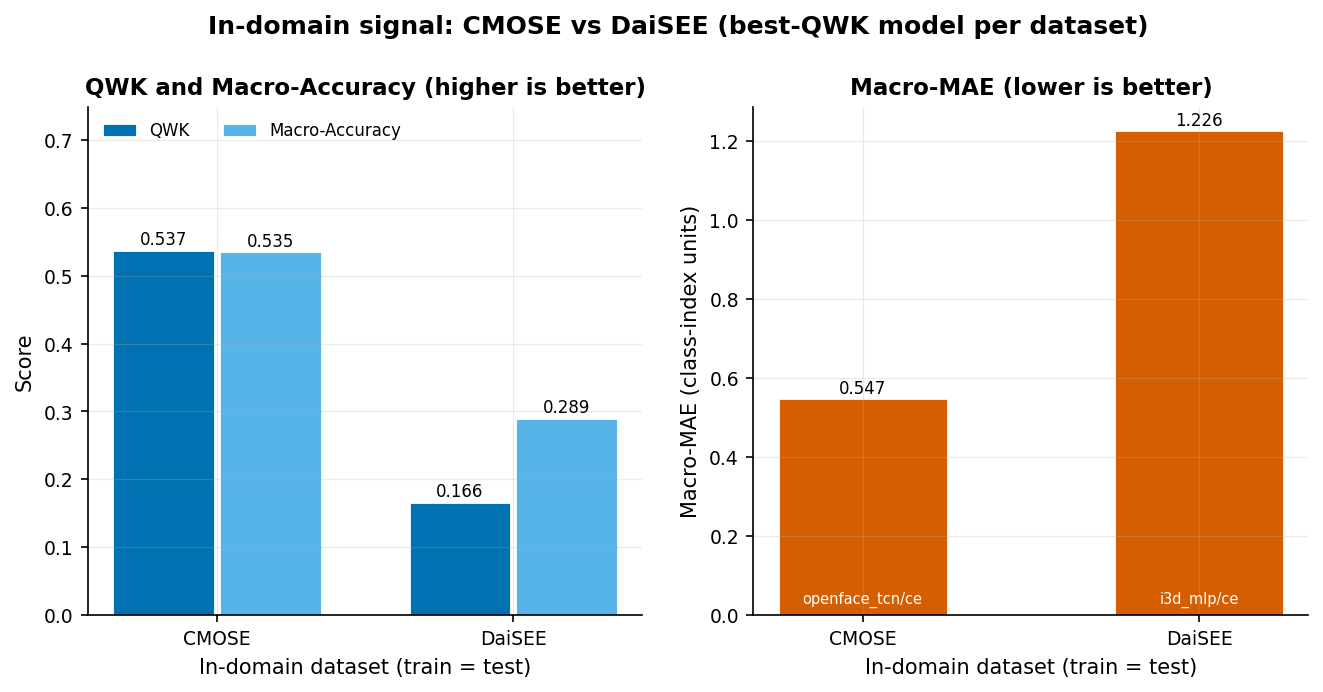
\includegraphics[width=0.9\linewidth]{figures/indomain_cmose_vs_daisee.png}
\caption{In-domain signal: CMOSE vs DaiSEE}
\label{fig:indomain_cmose_vs_daisee}
\end{figure}

\begin{figure}[ht]
\centering

\includegraphics[width=0.9\linewidth]{figures/loss_accuracy_tradeoff.png}
\caption{Accuracy vs macro-accuracy tradeoff by loss}
\label{fig:loss_accuracy_tradeoff}
\end{figure}

\begin{figure}[ht]
\centering

\includegraphics[width=0.9\linewidth]{figures/loss_curves_cmose_ce.png}
\caption{Loss curves cmose ce}
\label{fig:loss_curves_cmose_ce}
\end{figure}

\begin{figure}[ht]
\centering

\includegraphics[width=0.9\linewidth]{figures/per_class_f1.png}
\caption{Per-class F1: best base vs best hybrid}
\label{fig:per_class_f1}
\end{figure}

\begin{figure}[ht]
\centering
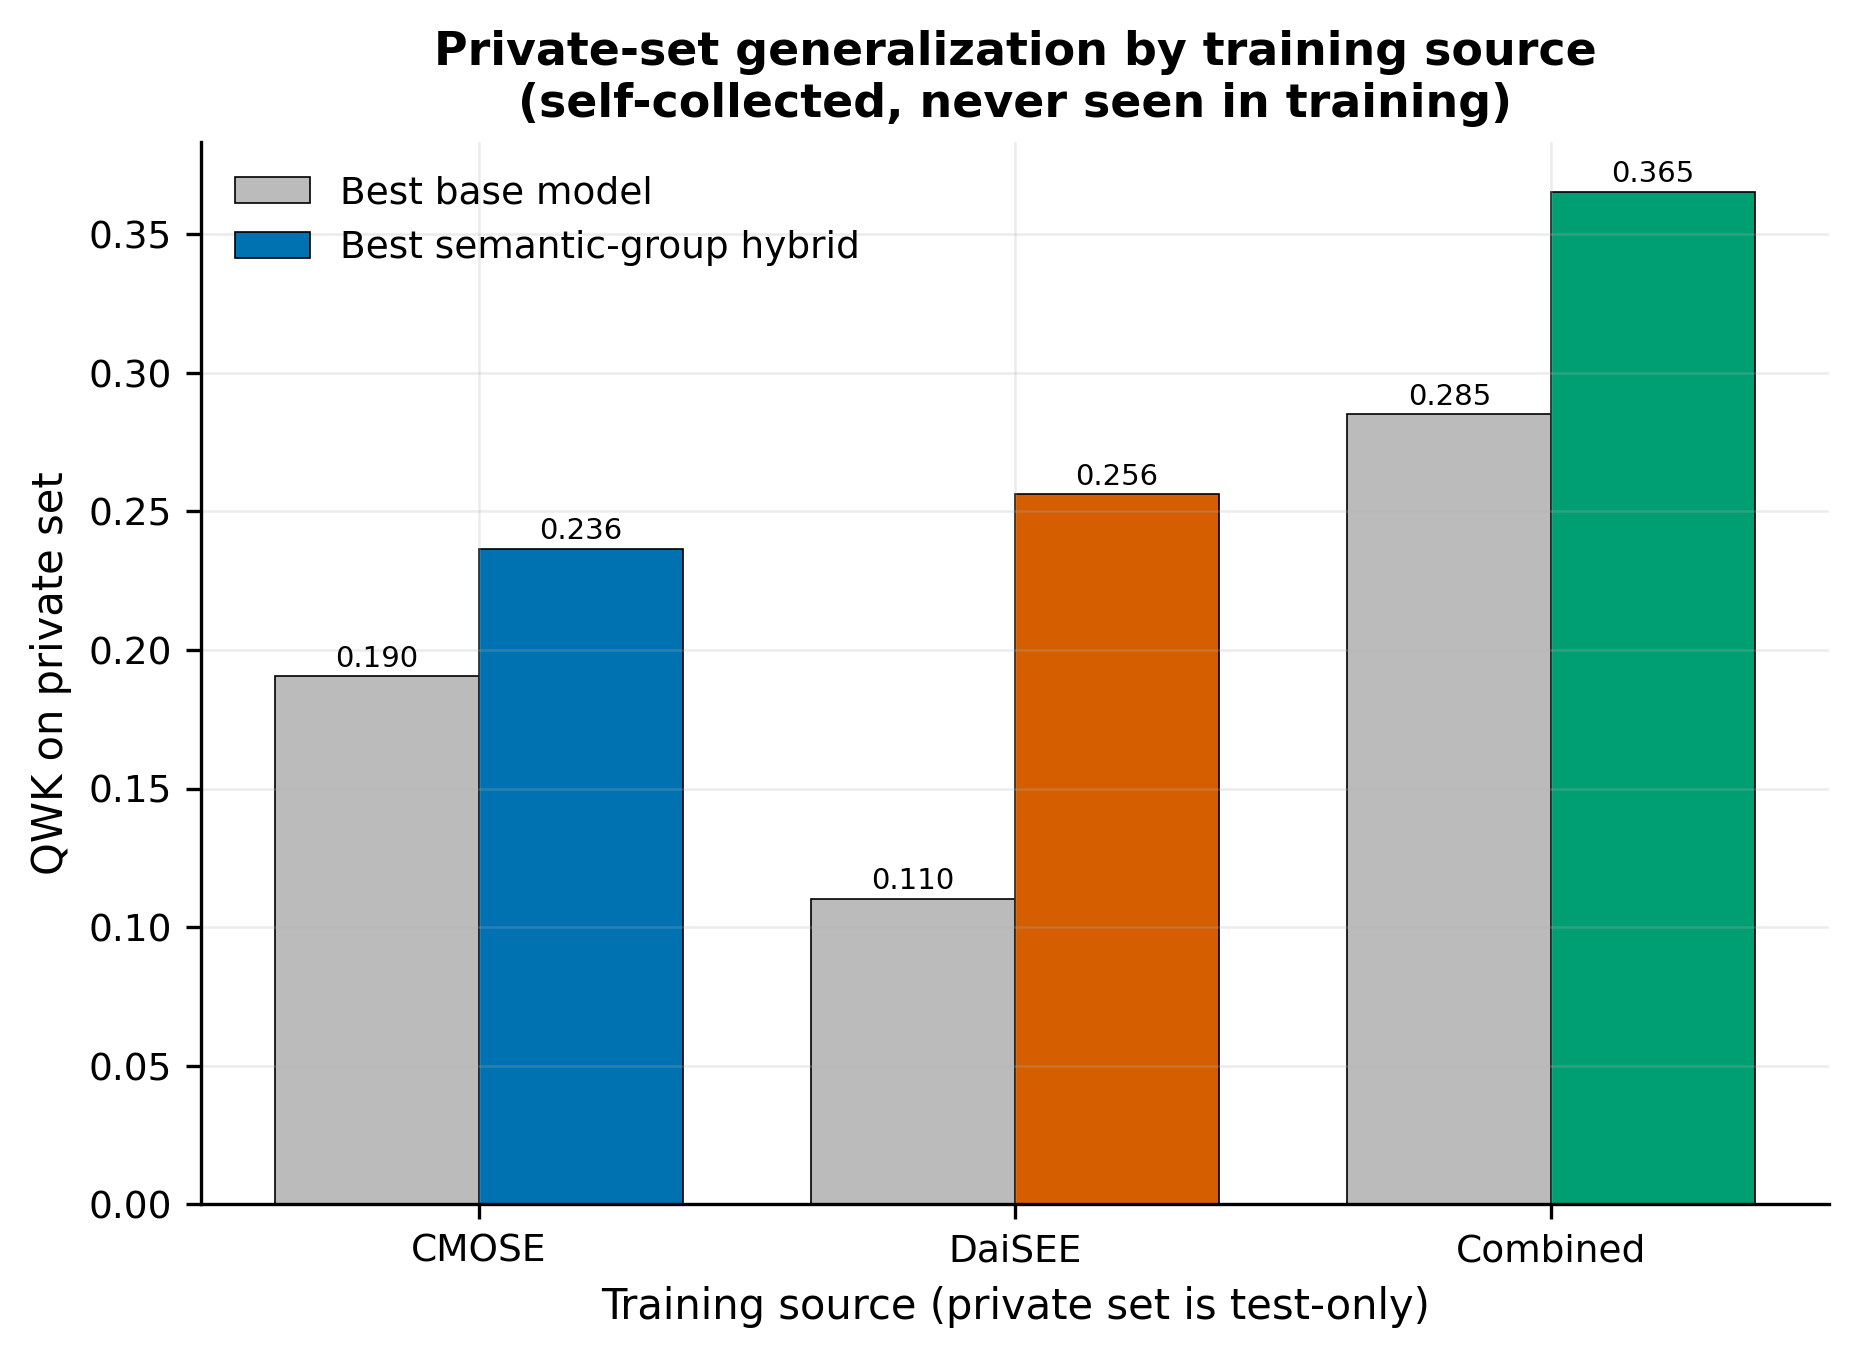
\includegraphics[width=0.9\linewidth]{figures/private_by_source.png}
\caption{Private-set generalization by training source}
\label{fig:private_by_source}
\end{figure}

\begin{figure}[ht]
\centering
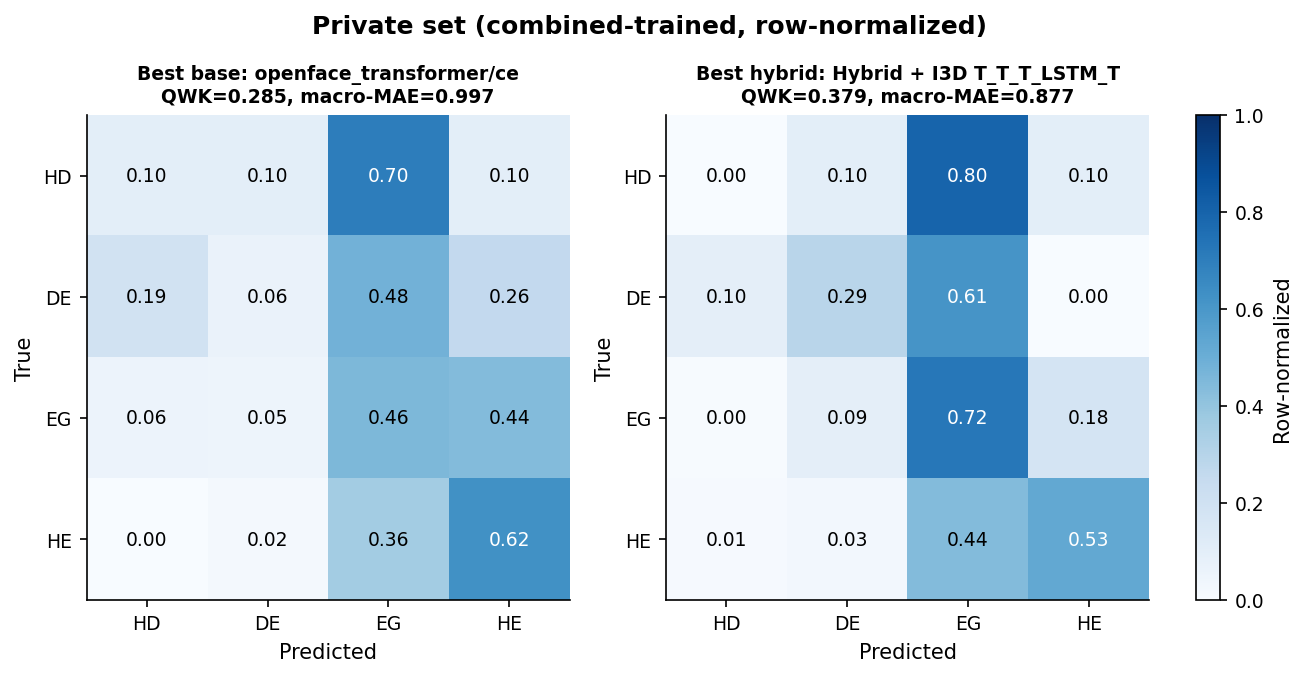
\includegraphics[width=0.9\linewidth]{figures/private_confusion_combined.png}
\caption{Private-set confusion, combined-trained I3D hybrid}
\label{fig:private_confusion_combined}
\end{figure}
